\documentclass[11pt]{article}
\usepackage{setspace}
\usepackage[a4paper,margin=1in]{geometry}
\geometry{margin=0.85in}
\setstretch{1.0}
\usepackage{graphicx}
\usepackage{array}
\usepackage{setspace}
\usepackage{parskip}
\usepackage{ragged2e}

\pagestyle{empty}
\setstretch{1.05}

\begin{document}


% Title
\begin{center}
    {\Large \textbf{Job Application}} \\[3cm]
    
    {\Huge \textbf{Zhongli Wang}} \\[0.4cm]
    
    {\LARGE Application for Associate, Regional Economist (Asia) \\ 
    \& Korea Economist}
\end{center}

\vspace{0.6cm}

% Large picture in the middle
\begin{center}
    \IfFileExists{../zhongli-wang-profile.jpg}{
        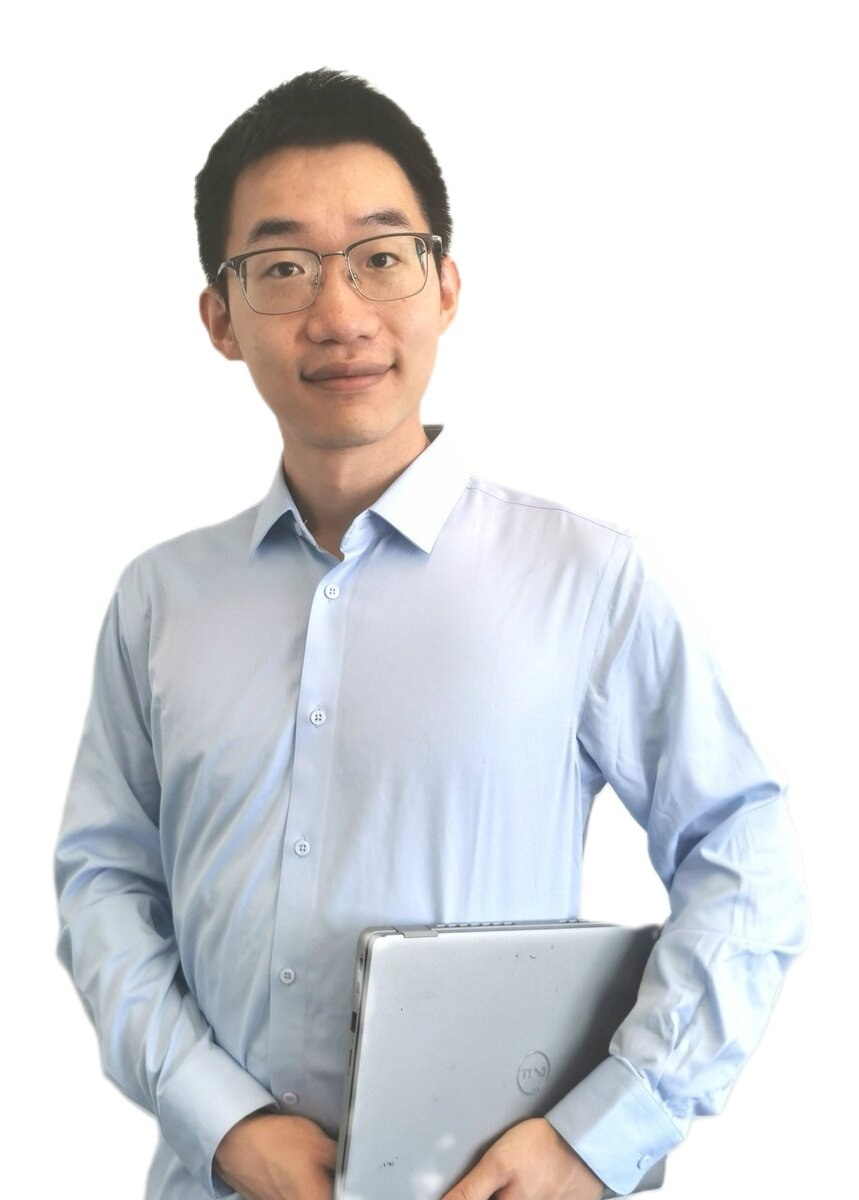
\includegraphics[
            width=0.55\textwidth,
            height=0.45\textheight,
            keepaspectratio
        ]{../zhongli-wang-profile.jpg}
    }{
        \vspace{0.45\textheight}
    }
\end{center}

\vspace{0.7cm}

% \vspace{3cm}


% Personal details
\begin{center}
\renewcommand{\arraystretch}{1.35}
\begin{tabular}{>{\bfseries}p{4.2cm} p{8.5cm}}


Address: & Astastrasse 22, 33617 Bielefeld, Germany \\

Number: & +49 160 9541 6015 \\

Email: & nkwangzhongli@gmail.com \\
\end{tabular}
\end{center}

\vfill

% \begin{center}
%     \small Last updated: \today
% \end{center}
\newpage
\enlargethispage{4\baselineskip}

\begin{flushright}
Zhongli Wang \\
Astastrasse 22 \\
33617 Bielefeld\\
Germany \\
\end{flushright}

\vspace{0.1cm}

\vspace{0.1cm}

\noindent
Bank of America, Global Research \\
Hong Kong SAR

\vspace{0.12cm}

\noindent
\textbf{Application for Associate, Regional Economist (Asia) \& Korea Economist}

\vspace{0.1cm}

\noindent Dear Bank of America Global Research recruiting team,

I recently completed my Ph.D. in Economics at Bielefeld University (defended on September 21, 2026),
and I hold an M.A. in Business and Economics with a major in Banking and Finance and a minor in Data Science,
along with a BSc in Finance from Nankai University. My doctoral research focuses on innovation policy,
data economics, and firm-level dynamics, providing a strong foundation for economic policy research
and economic forecasting in the Asian region. I also hold an approved Hong Kong Talent Pass, allowing
me to work in Hong Kong without additional visa sponsorship.

I am particularly drawn to the Regional Economist (Asia) \& Korea Economist role because it offers the opportunity
to conduct macroeconomic research on Asian economies with a concentration in Korea, and to develop independent
views on regional economic developments and their implications for equity, interest rate, and foreign exchange
markets. My background aligns closely with the position's requirements:

\begin{itemize}
    \item \textbf{Monetary policy and Asian economies:} I gained direct exposure to monetary policy implementation
    during my internship at the People's Bank of China, where I supported analysis of interest rate management,
    reserve requirements, and open market operations. This experience, combined with my BSc in Finance from Nankai
    University and native Mandarin Chinese proficiency, gives me strong grounding in Asian economic and financial
    market dynamics.
    \item \textbf{Econometric analysis and economic forecasting:} My doctoral research involves compiling and
    analyzing large economic datasets using Python and R, conducting econometric analysis, sensitivity analysis,
    and forecasting. I have published research in peer-reviewed finance journals, demonstrating the ability to
    produce rigorous written research and develop quantitative models.
    \item \textbf{Innovation policy and economic research:} My research examines innovation policy, data economics,
    and how heterogeneous consumers interact with the data value chain, which are topics at the intersection of economic
    policy and market dynamics that are increasingly relevant to Asian economies undergoing digital transformation.
    I have also developed AI-powered agentic workflows to automate economic research tasks including data
    compilation, analysis, and forecasting.
    % \item \textbf{Cross-country collaboration and communication:} I have collaborated with international research
    % teams across Germany, Italy, and Switzerland, presented findings at academic conferences, and communicated
    % economic research to both academic and practitioner audiences. I am comfortable working across countries,
    % functions, and time zones.
\end{itemize}

I have excellent command of English at C1 level, and I am a native Mandarin Chinese speaker with additional
proficiency in German (C1) and Cantonese (A2). I am highly motivated to apply my expertise in economic research,
econometrics, and Asian market knowledge to Bank of America's Asia economics team. I am eager to contribute to
research publications, develop independent economic forecasts for Korea and the broader Asian region, and
build strong relationships with internal and external clients.

Thank you so much for considering my application!
I would welcome the opportunity to discuss how my background and abilities could contribute to Bank of America's
Global Research team in Hong Kong.

% \vspace{0.08cm}
\noindent Kind regards, \\
\vspace{0.1cm}
\noindent
\includegraphics[width=2.7cm,keepaspectratio]{../Wang-sig.jpg} \\
\noindent Zhongli Wang


\end{document}
